\documentclass[10pt,letter,english]{article}

\usepackage{amsmath}
\usepackage{amscd}
\usepackage{amssymb}

\usepackage{tikz}
\usetikzlibrary{arrows}

\usepackage[sc,osf]{mathpazo}
\linespread{1.05}         % Palatino needs more leading (space between lines)
\usepackage[T1]{fontenc}
\fontencoding{T1}
\fontfamily{ppl}
\fontseries{m}
\fontshape{n}
\fontsize{10}{13}
\selectfont

%%%%%%%%%%%%%%%%%%%%%%%%%%%%%%%%%%%%%%%%%%%%%%%%%%%%%%%%%%%%%%%%%%%%%%%%%%%%%%%
%% Set Theory Concepts

\newcommand{\buildset}[2]{\{ #1 \;|\; #2 \}}
\newcommand{\compose}[0]{\circ}

\newcommand{\partto}{\rightharpoonup}

%%%%%%%%%%%%%%%%%%%%%%%%%%%%%%%%%%%%%%%%%%%%%%%%%%%%%%%%%%%%%%%%%%%%%%%%%%%%%%%
%% Textual Macros

\newcommand{\aam}[0]{\textsc{aam}}
\newcommand{\maam}[0]{\textsc{maam}}
\newcommand{\js}[0]{JavaScript}
\newcommand{\lambdajs}[0]{$\lambda_{JS}$}

%%%%%%%%%%%%%%%%%%%%%%%%%%%%%%%%%%%%%%%%%%%%%%%%%%%%%%%%%%%%%%%%%%%%%%%%%%%%%%%
%% Machine Configurations

\newcommand{\cek}[3]{\langle #1, #2, #3 \rangle}
\newcommand{\cesk}[4]{\langle #1, #2, #3, #4 \rangle}
\newcommand{\cessk}[5]{\langle #1, #2, #3, #4, #5 \rangle}
\newcommand{\cesskc}[6]{\langle #1, #2, #3, #4, #5, #6 \rangle}

%%%%%%%%%%%%%%%%%%%%%%%%%%%%%%%%%%%%%%%%%%%%%%%%%%%%%%%%%%%%%%%%%%%%%%%%%%%%%%%

\begin{document}

\title{MJSAI: Designing a Sound, Configurable, Efficient, and Pushdown %
              Monadic Static~Analyzer for JavaScript}
\author{{David Darais and Daniel King}\\
        School of Engineering and Applied Sciences\\
        Harvard University}

\maketitle

\section*{Abstract}

We present the design and implementation of a static analyzer for \js{}. We
leverage the Monadic Abstracting Abstract Machines (\maam{}) technique to create
an analysis which is both configurable and correct by construction. We recast
pushdown static analysis in terms of \aam{}. This recasting permits us to also
create a pushdown \maam{} analysis for \js{}.

\section{Introduction}

This work had three goals:

\begin{itemize}
\item design a configurable static analysis using the Monadic Abstracting
  Abstract Machines (\maam{}) technique
\item implement the analysis, again using the \maam{} technique
\item analyze the performance of many different analysis techniques, including
  pushdown analysis, against the JSAI \cite{jsai} benchmark suite
\end{itemize}

We completed most of the first two goals; however, we have not analyzed the
performance of the implementation. We underestimated the time necessary to
implement the JavaScript semantics in the \maam{} Huskily framework. We are also
currently unable to scale the analysis to real \js{} programs. Finally, we spent
a not insignificant amount of time understanding what pushdown analysis is and
how it can be implemented in the \aam{} and \maam{} frameworks.

The remainder of the paper presents the design and implementation of the
analysis, including subsections on our understanding of pushdown analysis.

\section{Design}
\subsection{Pushdown Analysis in MAAM}

Pushdown analysis means different things to different people. There is a
significant amount of work on first-order pushdown semantics, but we focus on
understanding the higher-order setting. There are primarily two papers which
describe a pushdown analysis for a higher-order setting: Vardoulakis and
Shivers' \emph{CFA2} \cite{cfa2} and Earl, Might, and Van Horn's \emph{PDCFA}
\cite{pdcfa}. Both papers share the idea of \emph{precise call-return matching}
and some form of \emph{memoization}. The former improves the precision and the
latter improves the time-efficiency of the analysis. The \emph{CFA2} analysis
also precisely tracks so-called \emph{stack} variables. We will not describe
this technique in detail other than to say that it involves identifying
variables which can safely live on the call stack and tracking their values
exactly. Unfortunately, even if one ignores the special \emph{stack} variables,
it is not obvious that the two techniques describe the same style of
analysis. The presentations styles differ dramatically: \emph{CFA2} describes a
Cousot \& Cousot style Abstract Interpretation whereas \emph{PDCFA} describes
the conversion of an abstract machine into a Dyck state graph.

We propose a unification of these two approaches using the \aam{} technique of
Might and Van Horn \cite{aam}. There are two simple ideas that lead to a
pushdown style analysis: a separate, path-sensitive store for continuations and
a memo table for function calls. We claim, without proof, that the
path-sensitive continuation-store provides \emph{precise call-return matching}.
The memo table for function calls clearly provides \emph{memoization}.

We can now describe a \aam{}-style approach for producing a pushdown abstract
machine from a concrete CEK machine:
\begin{enumerate}
\item Break recursion in the environment, caused by closures, with a store,
  which maps addresses to values, and change the environment to map variables to
  addresses.
\item Break recursion in the continuation stack by creating a
  continuation-store, which maps continuation-addresses to either the halt frame
  or a pair of a frame and a continuation-address.
\item Add a memo table which maps a triplets of a command, an environments, and
  a store to a value.
\end{enumerate}

\begin{figure}
\centering

\begin{equation*}
\begin{array}{c c l c l}
  c            &:& Exp        && \\
  \rho         &:& Env        &=& Var   \partto Addr \\
  \sigma       &:& Store      &=& Addr  \partto Value \\
  \kappa\sigma &:& KStore     &=& KAddr \partto Frame \times KAddr \\
  \kappa       &:& KAddr      && \\
  \chi         &:& Cache      &=& Exp \times Store \times Env \partto Value
\end{array}
\end{equation*}


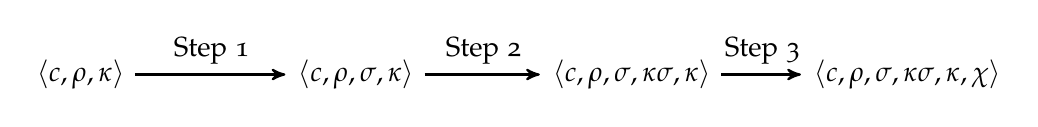
\begin{tikzpicture}[->,>=stealth',shorten >=1pt,auto,node distance=3.5cm,
  thick,main node/.style={font=\sffamily\bfseries}]

  \node[main node] (101) at (0, 1)
    {$\cek{c}{\rho}{\kappa}$};
  \node[main node] (102) [right of = 101]
    {$\cesk{c}{\rho}{\sigma}{\kappa}$};
  \node[main node] (103) [right of = 102]
    {$\cessk{c}{\rho}{\sigma}{\kappa\sigma}{\kappa}$};
  \node[main node] (104) [right of = 103]
    {$\cesskc{c}{\rho}{\sigma}{\kappa\sigma}{\kappa}{\chi}$};

  \path[->]
    (101) edge node {Step 1} (102)
    (102) edge node {Step 2} (103)
    (103) edge node {Step 3} (104);

\end{tikzpicture}
\caption{An AAM-style approach for producing a pushdown abstract machine} \label{fig:M1}
\end{figure}

\subsection{A JavaScript Analysis in MAAM}

\js{} has a large, complex specification and many implementations which
practically define the expected semantics of \js{}. Rather than describe and
implement our own semantics, we implement the \lambdajs{} semantics as described
in \cite{lambdajs}. Additionally, we reused their desugaring program.

We reformulated the \lambdajs{} semantics into a reduction machine
semantics. The \lambdajs{} evaluation contexts became our \emph{Frame} data
type. Additionally, we do not divide the evaluation contexts into two sets and
use syntactic stepping rules to implement exceptional control flow. We choose to
implement exceptional control flow with meta functions that crawl the stack
looking for appropriate return points.

\section{Implementation}



\section{Related Work}



\subsection{The Essence of JavaScript: \lambdajs{}}

The \lambdajs{} work provides a complete, practical foundation to perform
research on real-world JavaScript programs. The \lambdajs{} work identifies a
simplified language that captures the essential features of \js{}. The
\lambdajs{} language is the composition of four distinct semantics: function and
object semantics, mutable references, prototypal inheritance, and control
operators. In the authors' experience, implementing this semantics is time
consuming, but mindless. The complexity of \js{} is not apparent in the
\lambdajs{} model.

The complexity of \js{} is fully captured by a desugaring phase which replaces
certain forms, such as \texttt{with}, with simpler \js{} code. Additionally, the
\lambdajs{} team has an implementation of the \js{} standard library which
abstracts away the details of string and number coercions. These coercions are
specified by many pages of non-trivial pseudo-code in the ECMAScript 3rd Edition
standard.

\section{Conclusion}



\bibliography{paper}{}
\bibliographystyle{acm}

\end{document}
